\documentclass[25pt, a0paper, portrait, margin=0mm, innermargin=15mm, blockverticalspace=15mm, colspace=15mm, subcolspace=8mm]{tikzposter}

% define where to find graphics
\graphicspath{ {images/} {../design_document/images/} }

\usetheme{Wave}
\usebackgroundstyle{Rays}
\usenotestyle{Sticky}
\useblockstyle{TornOut}

% define size of poster
\geometry{paperwidth=36in,paperheight=48in}

\author{Timothy Dee, Justin Long, \& Brandon, McDonnel}

\title{Remotely Connected Electric Field Generator \\
for Particle Separation in a Fluid}

%\title{title}
%\author{author}
\institute{Team May1612}

\begin{document}

\maketitle

\begin{columns}
\column{.5}

\block{Minnetronix}
{
\begin{tikzfigure}
\includegraphics[width=0.2\textwidth]{images/minnetronix_logo.png}
\end{tikzfigure} 

% say something about Minnetronix
This project is sponsored by
Minnetronix, a health care company based in St. Paul, Minnesota,
founded in 1996.
Minnetronix continues to innovate landscape of health care technology
with an emphasis on device development and commercialization of medical technologies.
This project is apart of this effort.
%TODO
}

%
% Introduction
%
\block{Problem Statement}
{
% talk about dielectrophoresis
New research has shown that certain particles may be separated from fluids through dielectrophoresis.
This process involves applying an electric field to a fluid.
The electric field may then be manipulated in order to attract or repel certain particles.
The particles the electric field will attract or repel depends on
characteristics of the electric filed.
These field characteristics may be controlled
by varying the voltage and frequency 
of the electronics driving the field.

Our project is part of a larger design to 
exploit this phenomenon for use in medical equipment.
There are many medical applications which
utilize a method of separation.
Centrifuging blood and
testing spinal fluids are two examples of 
such systems.
Current testing equipment is expensive therefore
a cheaper device utilizing DEP would have 
a large competitive advantage if constructed. 
}

%\begin{subcolumns}
%\subcolumn{.5}

\block{Requirements}
{
%TODO expand upon these requirements
This device will need to be capable of operating in a laboratory environment.
It is also a great benefit if this device is portable.
%TODO
Given these constraints proposed solution seeks to create a device which is:
\begin{itemize}
\item small form factor
\item cheap
\item capable of separating particles in a fluid utilizing DEP
  \begin{itemize}
  \item produces $1$ to $60_{Vpp}$
  \item produces $10_{Khz}$ to $1_{Mhz}$
  \end{itemize}
\end{itemize}
}

%\subcolumn{.5}

\block{Solution}
{
To fulfill the requirements we propose the use of 
a Raspberry Pi in combination with 
some circuit components connected to the the GPIO pins
present on the Raspberry Pi.

%TODO insert picture of Raspberry Pi
%TODO describe what a Raspberry Pi is

The following components will be created and connected to the Raspberry Pi.
This will allow for the output of the circuit to be controlled using any computer on the LAN.
\begin{itemize}
\item Voltage Control
  \begin{itemize}
  \item Utilizes three Programmable Gain Amplifiers(PGA)
  \item Summing Amplifier to sum the output of PGA's
  \end{itemize}
\item Frequency Control
  \begin{itemize}
  \item Minigen Function Generator
  \item Communicates with Raspberry Pi through SPI
  \end{itemize}
\item Web Interface
  \begin{itemize}
  \item Apache 2 web server hosted on Raspberry Pi
  \item provides user ability to set voltage and frequency output
  \end{itemize}
\end{itemize}
}

%\end{subcolumns}

%
% Design Approach
%
\block{Block Diagram}
{
%TODO insert picture of block diagram
\begin{center}
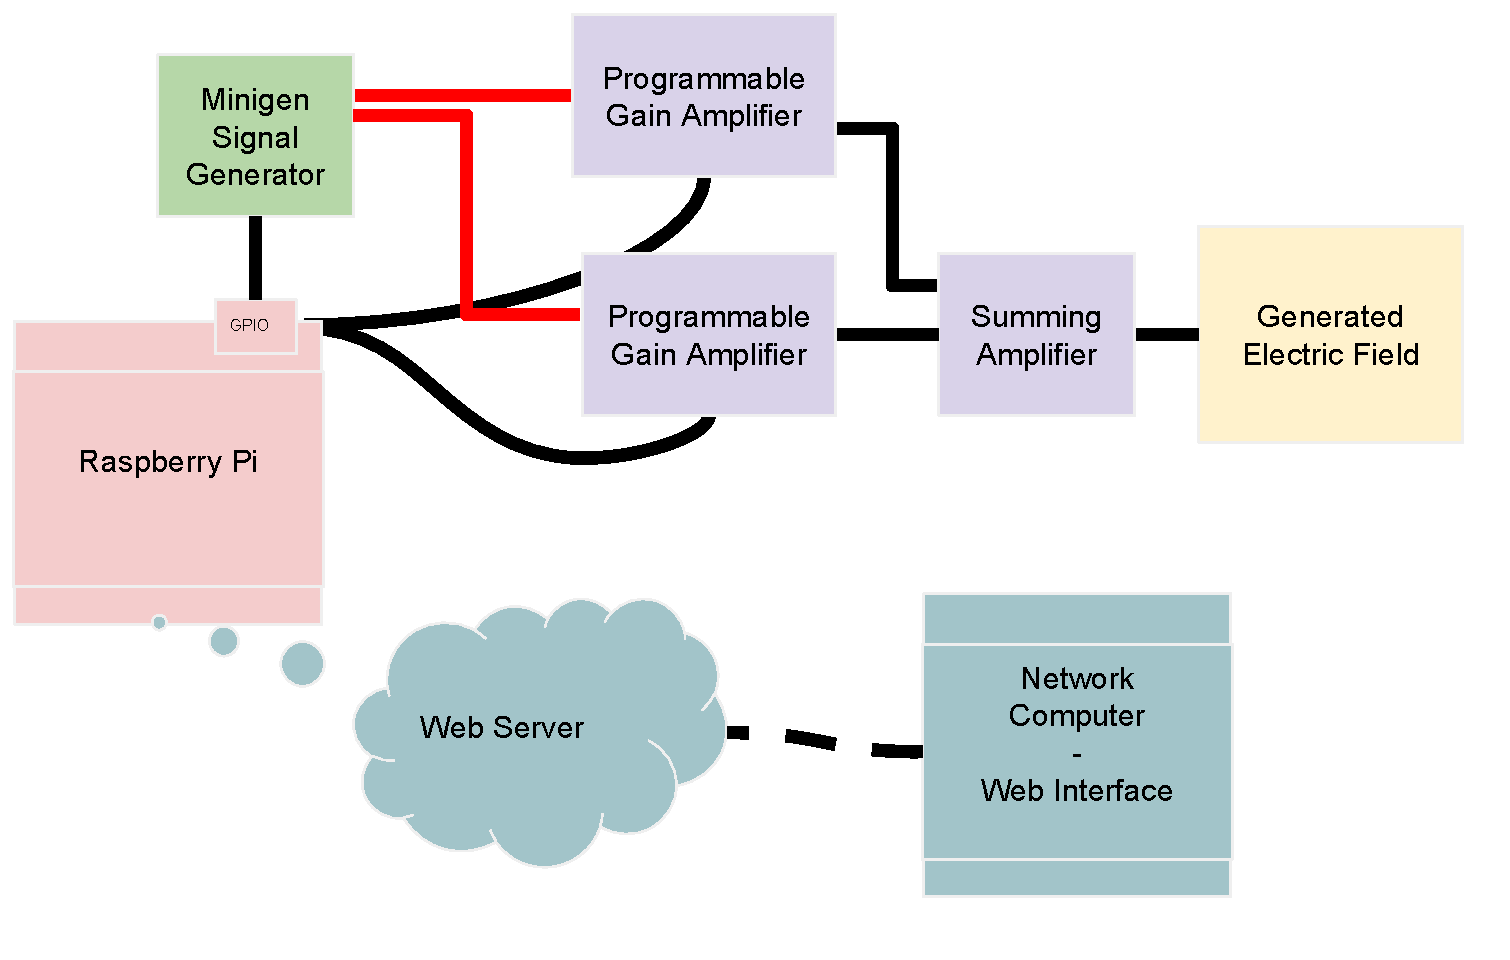
\includegraphics[width=0.35\textwidth,keepaspectratio]{block_diagram.png}
\end{center}

%TODO explain each of the functional modules
%TODO explain how each of the functional modules fit together
}

\column{.5}

%
% Technical Details
%
\block{Raspberry Pi}
{
The Raspberry Pi will act as the bridge between the user and the circuit.
The Raspberry Pi will host a web server allowing the user to interact with the system.
Based on the results of this user interaction, 
the Raspberry Pi will update the state of the GPIO pins.
The GPIO pins connect to a circuit causing the output to change based on their state. 

In addition to hosting the web server the Raspberry pi is used to
communicate with the 
Minigen Signal Generator and 
amplifier circuit.
This communication is accomplished via 
the Raspberry Pi's SPI interface and
GPIO pins respectively.

%TODO

%TODO insert Raspberry Pi connection diagram
\begin{center}
\includegraphics[width=0.35\textwidth,keepaspectratio]{rpi_connection.png}
\end{center}

%TODO insert picture of 
%TODO describe role in design 
\begin{itemize}
\item 
\end{itemize}
%TODO
}

\block{Web Interface}
{
The web interface is hosted on the Raspberry Pi using an Apache web server.
This web server displays an interface which allows the user to
set a voltage and frequency output by the system. 
The interface is simple and interactive,
implemented using cgi-scripts on the Apache web server.

Our implementation provides several functionalities.
Among these are
the ability to set:
voltage and frequency,
sine or triangle or square waveforms,
and the ability to set a voltage and frequency for an amount of time.
The table displayed
in the figure below
provides the ability to set voltage and frequency for the number
of minutes specified.
The "Go" button will cause the first
voltage and frequency to be set for the corresponding amount of time.
After the time has expired,
the next voltage and frequency will be set for the corresponding amount of time.
This process continues until the table entries are completed or
the user presses the "Stop" button.

\begin{center}
\includegraphics[width=0.35\textwidth,keepaspectratio]{491_web_interface_good.png}
\end{center}

%TODO insert picture of 
%TODO describe role in design 
\begin{itemize}
\item 
\end{itemize}
%TODO
}

\block{Minigen}
{
The Minigen Function Generator device controls the frequency output by the circuit.
Varying the frequency is accomplished 
by writing to registers present on the Minigen.
This communication is completed over SPI between
the Raspberry Pi and the Minigen.
The frequency produced is a function of
the values contained in the Minigen's frequency registers.

The Minigen outputs a waveform 
from -0.5V to 0.5V. 
This waveform may be a triangle, square, or sine wave.
The voltage output by the Minigen is not variable.
Given that the design specification requires a variable voltage,
the voltage needs to be adjusted separately.
Accordingly, the output of the Minigen 
is supplied to the input of the amplifier circuit.

The Minigen is controlled by setting five registers,
two registers for frequency, 
two for phase shift and 
one as a control. 
There exists no need for phase shifting
to meet the design requirements, 
however the frequency and control registers
are needed. 
By having two frequency registers,
data can be sent to one register while it is not in use,
followed by a write to the control register to use this register.
This allows for a nicer gradient, 
because the frequency will not change until the entire frequency register is written. 
The control register also allows for changing between sine, square and triangle waveforms.
In the event that the frequency needs to be finely adjusted,
this system utilizes the functionality of the control register
to modify the way in which writes to the frequency registers are received.
The way writes are received by the frequency registers 
can be varied between two modes.
In one mode,
two consecutive 14-bit writes to a frequency register are used.
In the other mode,
one write to the lower 14-bits of the 28-bit frequency register is used.
This functionality affords the ability to accurately dial in small changes to the register values quickly.

Until this point,
several functional benefits of the Minigen Signal Generator have been discussed.
An additional benefit which 
increases the practicality of this solution is the Minigen's small form factor.
The small chip size 
allows the Minigen to fit easily into a small case 
with the Raspberry Pi.
This is consistent with the system's requisite small footprint.

%TODO insert picture of 
%TODO describe role in design 
\begin{itemize}
\item 
\end{itemize}
%TODO
}

\block{Amplifier}
{
As mentioned in the previous section,
the output of the Minigen Function Generator
is applied to the amplifier circuit as input.
The amplifier also receives input from 
the GPIO pins of the Raspberry Pi.
These GPIO pins act as switches which help to control the output voltage.
Based on these inputs 
the amplifier circuit manages the overall 
voltage and frequency output.

The project requirements state that the system must 
generate signals which range from $1V_{pp}$ to $60V_{pp}$. 
To accomplish this,
various circuit components were used to accomplish the amplification.
The overall scheme is to split the output voltages into
three different ranges.
One component is used to adjust the voltage within each of the ranges while
other comp are used to change the range the voltage adjuster is acting within.

%TODO insert picture of 
%TODO describe role in design 
\begin{itemize}
\item 
\end{itemize}
%TODO
}

%
% Testing
%
\block{Testing}
{
%TODO include picture
%TODO explain testing environment
A typical testing environment includes:
\begin{itemize}
\item Oscilloscope
\item Raspberry Pi
  \begin{itemize}
  \item Connected for monitor for web interface access
  \item Connected to circuit to control Minigen, PGA's
  \end{itemize}
\item Multiple breadboards
  \begin{itemize}
  \item Minigen Function Generator
  \item PGA's
  \item Summing amplifier
  \end{itemize}
\end{itemize}

%TODO explain testing strategy
Testing this project involved
and iterative process of:
\begin{enumerate}
\item Theorize a design
\item Acquire necessary components
\item Construct design
\item Understand problems
\item Return to step 1
\end{enumerate}
Many times we found that designs would not work
and thus this process began at the beginning.
}

\end{columns}
\end{document}